\documentclass{beamer}
\usetheme{Warsaw}
\usecolortheme{crane}
\title[DOCUMENT SPELL CHECKER]{SPELL CHECKER}
\author{George Puthanangadi}

\institute{Federal Institute Of Science And Technology}
\date{October 2019}
\usepackage{graphicx}
\begin{document}
\begin{frame}
\titlepage
\end{frame}
\begin{frame}
\begin{enumerate}
\item Aim
\item Introduction
\item Existing Algorithm-1
\item Existing Algorithm-2
\item Proposed Method
\item Proposed Architecture
\item Proposed flowchart
\item Result
\item Conclusion
\end{enumerate}
\end{frame}
\begin{frame}{AIM}
writing a spell checker program to check the correctness of a given document
\end{frame}
\begin{frame}{INTRODUCTION}
We have to create a user program that checks the correctness of a document and makes neccesary changes if needed.Spell-checking features are often embedded in software or services, such as a word processor, email client, electronic dictionary, or search engine. 
\end{frame}
\begin{frame}{EXISTING ALGORITHM PAGE 1-Grammerly}
 Grammarly is an AI powered tool.
 \begin{enumerate}
 
 

\item So it’s basically a computer program or algorithm  which studies and compares your sentence against hundreds of similar ones that are listed in their database.
\item Grammarly, as mentioned earlier, is an AI powered tool that weighs your writing by comparing it against authentic rules and sentence patterns
\item Grammarly’s algorithms flag potential issues in the text and suggest context-specific corrections for grammar, spelling and usage, wordiness, style, punctuation, and even plagiarism using patterns in its database.

\end{enumerate}

\end{frame}
\begin{frame}

\includegraphics[scale=0.5]{grammer.png} 
\end{frame}

\begin{frame}{EXISTING ALGORITHM PAGE 2-GINGER}
 Ginger Software is an Israeli start-up company.
 \begin{enumerate}
 
 \item Ginger Software that has developed language enhancement technology that uses statistical algorithms in conjunction with natural language processing

\item Ginger Software uses patented software algorithms that deal with natural language processing. The company claims that the algorithm allows it to correct the written sentences with relatively high accuracy (eliminating up to 95 percent of writing errors) compared to standard spell checkers. \item Its unique algorithm allows the software to understand the context of the sentence rather than correcting based solely on a word. 
\item The software operates on the logic of sentence context in addition to the memory of a database of words.

\end{enumerate}

\end{frame}
\begin{frame}

\includegraphics[scale=0.5]{ginger.jpeg} 
\end{frame}



\begin{frame}{PROPOSED METHODOLOGY}
To do the User Authentication we use
\begin{enumerate}
\item online Dictionary
\item where we cross check word ny word with its counterpart in the dictionary using the first letter as hint.
\end{enumerate}
\end{frame}
\begin{frame}{Proposed algorithm}
 \begin{enumerate}
 
 \item Given document is broken down into words and duplicate words are removed.
\item each word os checked up in the dictionary module and f found is kept or else added t the dictionary if needed or changed by the user if not needed. 
\item the final edition is done by the user and r=corrected document is received

\end{enumerate}

\end{frame}

\begin{frame}{FLOW CHART}
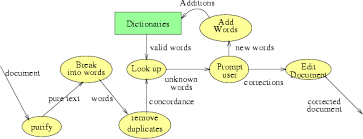
\includegraphics[scale=0.5]{index.png}     
\end{frame}



\begin{frame}{CONCLUSION}
A spell checker has been created where words are cross hecked in a online dictionary for mispellings and are corrected if possible.

\end{frame}

\end{document}
